\documentclass[journal]{IEEEtran}

\usepackage{adjustbox}
\usepackage{algorithm}
\usepackage{algpseudocode}
\usepackage{amsfonts}
\usepackage{amsmath}
\usepackage{amssymb}
\usepackage{amsthm}
\usepackage{array}
\usepackage{circuitikz}
\usepackage{cite}
\usepackage{colortbl}
\usepackage{environ}
\usepackage{fixmath}
\usepackage{grffile}
\usepackage{hyperref}
\usepackage{import}
\usepackage{mathtools}
\usepackage{microtype}
\usepackage{multirow}
\usepackage{pgffor}
\usepackage{pgfgantt}
\usepackage{pgfplots}
\usepackage{physics}
\usepackage{siunitx}
\usepackage{stfloats}
\usepackage{tcolorbox}
\usepackage{tikz}
\usepackage{url}
\usepackage{xcolor}
\usepackage[T1]{fontenc}
\usepackage[acronym]{glossaries-extra}
\usepackage[caption=false,font=footnotesize,subrefformat=parens,labelformat=parens]{subfig}
\usepackage[short]{optidef}
\usepackage[subtle]{savetrees}

\listfiles
\interdisplaylinepenalty=2500
\pgfplotsset{compat=newest}
\usepgfplotslibrary{patchplots}
\newtheorem{proposition}{Proposition}
\newtheorem{remark}{Remark}
\newtheorem{theorem}{Theorem}
\DeclareSIUnit{\belm}{Bm}
\DeclareSIUnit{\dBm}{\deci\belm}
\DeclareSIUnit{\beli}{Bi}
\DeclareSIUnit{\dBi}{\deci\beli}
\ctikzset{american}
\usetikzlibrary{arrows,calc,matrix,patterns,positioning}

\DeclarePairedDelimiterX{\infdivx}[2]{(}{)}{%
	#1\;\delimsize\|\;#2%
}
\newcommand{\infdiv}{D\infdivx}
\renewcommand{\qedsymbol}{\hfill\ensuremath{\Box}}

\makeatletter
\tikzset{
	block/.style={draw,rectangle,align=center},
    from/.style args={#1 to #2}{
        above right={0cm of #1},
        /utils/exec=\pgfpointdiff
            {\tikz@scan@one@point\pgfutil@firstofone(#1)\relax}
            {\tikz@scan@one@point\pgfutil@firstofone(#2)\relax},
        minimum width/.expanded=\the\pgf@x,
        minimum height/.expanded=\the\pgf@y
	}
}
\makeatother

\algrenewcommand{\algorithmicwhile}{\textbf{While}}
\algrenewcommand{\algorithmicif}{\textbf{If}}
\algrenewcommand{\algorithmicthen}{\textbf{Then}}
\algrenewcommand{\algorithmicelse}{\textbf{Else}}
\algrenewcommand{\algorithmicend}{\textbf{End}}
\algrenewcommand{\algorithmicrepeat}{\textbf{Repeat}}
\algrenewcommand{\algorithmicuntil}{\textbf{Until}}

\setabbreviationstyle[acronym]{long-short}

\newacronym{af}{AF}{Amplify-and-Forward}
\newacronym{ambc}{AmBC}{Ambient Backscatter Communications}
\newacronym{ap}{AP}{Access Point}
\newacronym{awgn}{AWGN}{Additive White Gaussian Noise}
\newacronym{bcd}{BCD}{Block Coordinate Descent}
\newacronym{bibo}{BIBO}{Binary-Input Binary-Output}
\newacronym{bpcu}{\si{bpcu}}{bit per channel use}
\newacronym{bpsphz}{\si{bps/Hz}}{bit per second per Hertz}
\newacronym{cscg}{CSCG}{Circularly Symmetric Complex Gaussian}
\newacronym{csi}{CSI}{Channel State Information}
\newacronym{df}{DF}{Decode-and-Forward}
\newacronym{dmc}{DMC}{Discrete Memoryless Channel}
\newacronym{dmtc}{DMTC}{Discrete Memoryless Thresholding Channel}
\newacronym{dmtmac}{DMTMAC}{Discrete Memoryless Thresholding Multiple Access Channel}
\newacronym{dp}{DP}{Dynamic Programming}
\newacronym{iid}{i.i.d.}{independent and identically distributed}
\newacronym{irs}{IRS}{Intelligent Reflecting Surface}
\newacronym{kkt}{KKT}{Karush–Kuhn–Tucker}
\newacronym{mac}{MAC}{Multiple Access Channel}
\newacronym{mc}{MC}{Multiplication Coding}
\newacronym{miso}{MISO}{Multiple-Input Single-Output}
\newacronym{mimo}{MIMO}{Multiple-Input Multiple-Output}
\newacronym{ml}{ML}{Maximum-Likelihood}
\newacronym{noma}{NOMA}{Non-Orthogonal Multiple Access}
\newacronym{ofdm}{OFDM}{Orthogonal Frequency-Division Multiplexing}
\newacronym{pdf}{PDF}{Probability Density Function}
\newacronym{psk}{PSK}{Phase Shift Keying}
\newacronym{pin}{PIN}{Positive Intrinsic-Negative}
\newacronym{qam}{QAM}{Quadrature Amplitude Modulation}
\newacronym{rf}{RF}{Radio Frequency}
\newacronym{sc}{SC}{Superposition Coding}
\newacronym{sic}{SIC}{Successive Interference Cancellation}
\newacronym{simo}{SIMO}{Single-Input Multiple-Output}
\newacronym{sinr}{SINR}{Signal-to-Interference-plus-Noise Ratio}
\newacronym{smawk}{SMAWK}{Shor-Moran-Aggarwal-Wilber-Klawe}
\newacronym{sr}{SR}{Symbiotic Radio}
\newacronym{tdma}{TDMA}{Time-Division Multiple Access}
\newacronym{tg}{TG}{tag}
\newacronym{ue}{UE}{user}


\begin{document}
\title{Metascatter: Unifying Symbiotic Radio and Intelligent Reflecting Surface}
\author{
	\IEEEauthorblockN{
		Yang~Zhao,~\IEEEmembership{Member,~IEEE,}
		and~Bruno~Clerckx,~\IEEEmembership{Senior~Member,~IEEE}
	}
	\thanks{
		The authors are with the Department of Electrical and Electronic Engineering, Imperial College London, London SW7 2AZ, U.K. (e-mail: \{yang.zhao18, b.clerckx\}@imperial.ac.uk).
	}
}
\maketitle

\begin{abstract}
	Backscatter allows wireless nodes to harvest energy from, modulate information over, and reconfigure propagation of surrounding radio waves.
	We introduce the concept of Metascatter, which adapts the input probability distribution of a finite-state backscatter device based on Channel State Information (CSI), to simultaneously act as parasitic source of Symbiotic Radio (SR) that conveys sensor data and reflecting element of Intelligent Reflecting Surface (IRS) that assists legacy transmission.
	Using shared spectrum, energy, and infrastructures, fully cognitive networks can be built over Metascatter, and we consider a basic scenario where a multi-antenna Access Point (AP) and multiple Metascatter simultaneously transmit to a single-antenna user.
	Since tags involve load switching and the primary and backscatter messages are multiplied (instead of superposed) in the received signal, it is assumed the user employ joint energy detection on all tags, then model their reflection pattern within the equivalent CSI for primary decoding.
	We characterize the achievable primary-(sum-)backscatter rate region through a joint optimization of transmit beamforming vector at the AP, input probability distribution at the tags, and energy detection regions at the user.
	A suboptimal solution is provided by the Block Coordinate Descent (BCD) method, where the beamforming, input distribution, and decision thresholds are obtained by Successive Convex Approximation (SCA), Karush–Kuhn–Tucker (KKT), and Dynamic Programming (DP), respectively.
	Simulation results demonstrate Metascatter can exploit the additional backscatter path to transmit and assist.
\end{abstract}

\begin{section}{Introduction}
	\IEEEPARstart{B}{ackscatter} is recently re-innovated as a promising approach to support low-power communications and control wireless propagation environments.
	The concept of \gls{ambc} was first proposed in \cite{Liu2013b}, where each tag harvests energy from and modulates information over ambient \gls{rf} signals by periodically switching between different reflection patterns.
	It enables battery-free communication between fully passive nodes, but the backscatter signal strength can be relatively weak and the decoding is subject to strong direct-link interference.
	To solve this, \cite{Yang2018d} exploited the repeating structure of \gls{ofdm} symbol for interference cancellation based on backscatter channel strength.
	Cooperative primary-backscatter decoding using co-located receiver, known as cooperative \gls{ambc}, was proposed in \cite{Yang2018}.
	The authors evaluated the error performance of \gls{ml}, linear, and \gls{sic} detectors for flat fading channels, and proposed a low-complexity \gls{ml} detector for frequency-selective fading channels with ambient \gls{ofdm} carrier.
	When transmit cooperation is also available, cooperative \gls{ambc} is more commonly known as \gls{sr} \cite{Liang2020}.
	The authors of \cite{Guo2019b} classified \gls{sr} into commensal, parasitic, and competitive modes based on the relative link priority, then derived their instantaneous achievable rate and optimal power allocation.
	The outage probability for those modes was later studied in \cite{Ding2020}.
	On the other hand, it was concluded in \cite{Long2020a} that if the backscatter symbol period is much longer than the primary symbol period, then the non-coherent achievable rate of primary decoding would approach that of the coherent case.
	The authors also considered the transmit precoder design for weighted sum-rate maximization and transmit power minimization problems.
	\cite{Zhou2019a} explored how the number of transmit antennas, receive antennas, and symbol period ratio asymptotically influence the ergodic rate of primary and backscatter links.
	With multi-antenna at all ends, \cite{Wu2021a} optimized the transmit precoder to maximize the backscatter achievable rate under primary rate constraint.
	However, those paper only considered single tag scenario and the optimal tag multiple access scheme remains unknown.
	\cite{Xu2021a} proposed a \gls{noma}-based \gls{sr} and studied the receive combiner design when the receiver decodes in the order of equivalent channel strength.
	A \gls{tdma}-based \gls{sr} with energy harvesting constraints was also presented in \cite{Yang2021a}, and energy efficiency maximization was considered with respect to transmit power, reflection efficiency, and time allocation design.
	In \cite{Han2021}, random code-assisted backscatter multiple access was combined with \gls{sr}, and the authors evaluated the asymptotic \gls{sinr} performance using random matrix theory.

	On the other hand, \gls{irs} has recently emerged as a promising technique to enhance the energy efficiency.
	In practice, an \gls{irs} consists of multiple individual sub-wavelength reflecting elements to adjust the amplitude and phase of the incoming signal (i.e., passive beamforming).
	Different from relay, backscatter and frequency-selective surface \cite{Anwar2018}, \gls{irs} assists the primary transmission using passive components with much lower energy consumption and thermal noise, but is limited to frequency-dependent reflection.
	\cite{Wu2018} proposed an \gls{irs}-assisted \gls{miso} system and jointly optimized the precoder and the phase shifts to minimize the transmit power.
	The active and passive beamforming problem was then extended to the discrete phase shift case \cite{Wu2019a} and the multi-user case \cite{Wu2019}.
	In \cite{Abeywickrama2020}, the authors investigated the impact of non-zero resistance on the reflection pattern and emphasized the coupling between reflection amplitude and phase shift in practice.
	To estimate the cascaded link without \gls{rf}-chains at the \gls{irs}, practical protocols were developed based on element-wise on/off switching \cite{Nadeem2019}, training sequence and reflection pattern design \cite{You2019,Kang2020}, and compressed sensing \cite{Wang2020}.
	\gls{irs} was also added to single-tag and multi-tag \gls{sr} systems to improve backscatter efficiency \cite{Chen2021,Zhang2021d}.
	Recently, the idea of \gls{irs}-empowered \gls{sr} was proposed in \cite{Xu2020b,Hua2022}, where the reflection pattern can be decoupled as the multiplication of whole phase shift matrix and one backscatter symbol.
	The idea was combined with spatial modulation to divide the \gls{irs} into reflection and information and elements, and the error performance of non-coherent backscatter detection was studied accordingly \cite{Hu2021a}.

	To the best of our knowledge, most existing \gls{sr} systems \cite{Yang2018,Guo2019b,Ding2020,Long2020a,Zhou2019a,Wu2021a,Xu2021a} assumed Gaussian codebook at the tags and employed \gls{sic} from primary to backscatter link.
	It thus requires non-coherent primary encoding at the transmitter and involves re-encoding, precoding, and subtraction operations that may not be available to legacy receivers.
	Besides, the primary and backscatter symbols in \gls{sr} are mixed by multiplication coding instead of superposition coding, and the backscatter symbol period can be much longer than the primary symbol period due to physical constraints.
	Inspired by above, we propose a novel Metascatter network where multiple battery-free tags ride over a conventional point-to-point system and adapt their input probability distribution to simultaneously act as backscatter tags of \gls{sr} and reflecting elements of \gls{irs}.
	To fully utilize the reflection pattern and signal structure, we also present a novel decoding strategy with minor modifications on existing receivers.
	The contributions of this paper is summarized as follows.


	\emph{First,} Metascatter adapts the input probability distribution of a finite-state backscatter device based on the primary and backscatter \gls{csi}.
	It generalizes the backscatter tags of \gls{sr} and reflecting elements of \gls{irs} to improve the primary-backscatter tradeoff in a flexible manner.
	When the primary link is absolutely prioritized, the tag input probability boils down to \num{1} at the state that maximizes the equivalent channel strength and \num{0} at other states, which is essentially the phase shift selection of an \gls{irs} element.
	When we only care about the backscatter performance, the network boils down to a multi-tag \gls{ambc} and the input design can be simplified accordingly.

	\emph{Second,} we propose a novel receiving strategy where the backscatter symbol of all tags are first recovered by energy-based decoding, then modeled within equivalent \gls{csi} for primary decoding.
	When the ratio of backscatter symbol period over primary symbol period is large enough, the randomness of primary source can be averaged out and the performance of non-coherent backscatter decoding can be greatly improved.
	Since the primary and backscatter symbols are mixed by multiplication coding, the backscatter decoding can be viewed as part of primary channel training, which avoids non-coherent encoding at the transmitter and \gls{sic} at the receiver.

	\emph{Third,} we characterize the achievable primary-(sum-)backscatter rate region by iteratively optimizing the tag input distribution, the backscatter decision threshold, and the transmit precoder.
	For the input design, we propose a numerical method to evaluate the \gls{kkt} solutions by limits of sequences.
	For the threshold design, we derive the minimum number of decision thresholds to maximize the total backscatter rate, and obtain the optimal thresholds by \gls{dp} accelerated by \gls{smawk} algorithm.
	However, the optimal precoder design can be non-trivial and we may end up with a low-complexity suboptimal solution.

\end{section}

\begin{section}{Backscatter Principles}
	% \begin{figure}[!t]
	% 	\centering
	% 	\resizebox{0.6\columnwidth}{!}{
	% 		\begin{circuitikz}[transform shape]
	% 			\coordinate (O) at (0,0);
	% 			\node[block,from={O to $(O) + (6.375,3.25)$}](T){};
	% 			\draw (0,1.75)
	% 			to[short] ++(-0.875,0)
	% 			to[short] ++(0,0.5) node[bareantenna](A){Bx};
	% 			\draw (0,1.75)
	% 			to[short,-*] ++(0.25,0) coordinate(J);
	% 			\draw (J)
	% 			to[short] ++(0,1)
	% 			to[short] ++(0.5,0) coordinate(J1);
	% 			\node[block,from={$(J1) + (0,-0.25)$ to $(J1) + (2.5,0.25)$}](R){Rectifier};
	% 			\draw (J)
	% 			to[short] ++(0.5,0) coordinate(J2);
	% 			\node[block,from={$(J2) + (0,-0.25)$ to $(J2) + (2.5,0.25)$}](D){Demodulator};
	% 			\draw (J)
	% 			to[short] ++(0,-1)
	% 			to[short] ++(0.5,0) coordinate(J3)
	% 			to [vR,mirror,invert,/tikz/circuitikz/bipoles/length=1cm] ++(1.75,0) node[ground,rotate=90]{};
	% 			\node[block,from={$(J3) + (0,-0.25)$ to $(J3) + (2.5,0.25)$},draw=none](M){};
	% 			\draw ($(J3) + (0,-0.25)$) rectangle ($(J3) + (2.5,0.25)$);
	% 			\draw ($(J3) + (1.25,-0.5)$) node[]{Modulator};
	% 			\draw[dashed,-{Latex[length=2mm]}] (R.east) -- ++(0.75,0);
	% 			\draw[-{Latex[length=2mm]}] (D.east) -- ++(0.75,0);
	% 			\draw[{Latex[length=2mm]}-] (M.east) -- ++(0.75,0);
	% 			\node[block,from={$(R.east) + (0.75,-0.25)$ to $(R.east) + (2.875,0.25)$}](P){Power buffer};
	% 			\node[block,from={$(M.east) + (0.75,-0.25)$ to $(D.east) + (2.875,0.25)$}](S){Digital\\section};
	% 			\draw[dashed,-{Latex[length=2mm]}] (P.south) to (S.north);
	% 			\coordinate (F1) at ($(P.south)!0.5!(S.north)$);
	% 			\coordinate (F2) at ($(D.east)!0.5!(S.west)$);
	% 			\coordinate (F3) at ($(D.south)!0.5!(M.north)$);
	% 			\draw[dashed] (F1) to (F1-|D.north);
	% 			\draw[dashed,-{Latex[length=2mm]}] (F1-|D.north) to (D.north);
	% 			\draw[dashed] (F1-|F2) to (F2|-F3) to (M|-F3);
	% 			\draw[dashed,-{Latex[length=2mm]}] (M|-F3) to (M.north);
	% 		\end{circuitikz}
	% 	}
	% 	\caption{The block diagram and equivalent circuit of a passive tag. The solid and dashed vectors represent signal and energy flows.}
	% 	\label{fi:tag_block_diagram}
	% \end{figure}

	\begin{figure}[!t]
		\centering
		\subfloat[Block diagram]{
			\resizebox{0.6\columnwidth}{!}{
				\begin{circuitikz}[transform shape]
					\coordinate (O) at (0,0);
					\node[block,from={O to $(O) + (6.375,3.25)$}](T){};
					\draw (0,1.75)
					to[short] ++(-0.875,0)
					to[short] ++(0,0.5) node[bareantenna](A){Bx};
					\draw (0,1.75)
					to[short,-*] ++(0.25,0) coordinate(J);
					\draw (J)
					to[short] ++(0,1)
					to[short] ++(0.5,0) coordinate(J1);
					\node[block,from={$(J1) + (0,-0.25)$ to $(J1) + (2.5,0.25)$}](R){Rectifier};
					\draw (J)
					to[short] ++(0.5,0) coordinate(J2);
					\node[block,from={$(J2) + (0,-0.25)$ to $(J2) + (2.5,0.25)$}](D){Demodulator};
					\draw (J)
					to[short] ++(0,-1)
					to[short] ++(0.5,0) coordinate(J3)
					to [vR,mirror,invert,/tikz/circuitikz/bipoles/length=1cm] ++(1.75,0) node[ground,rotate=90]{};
					\node[block,from={$(J3) + (0,-0.25)$ to $(J3) + (2.5,0.25)$},draw=none](M){};
					\draw ($(J3) + (0,-0.25)$) rectangle ($(J3) + (2.5,0.25)$);
					\draw ($(J3) + (1.25,-0.5)$) node[]{Modulator};
					\draw[dashed,-{Latex[length=2mm]}] (R.east) -- ++(0.75,0);
					\draw[-{Latex[length=2mm]}] (D.east) -- ++(0.75,0);
					\draw[{Latex[length=2mm]}-] (M.east) -- ++(0.75,0);
					\node[block,from={$(R.east) + (0.75,-0.25)$ to $(R.east) + (2.875,0.25)$}](P){Power buffer};
					\node[block,from={$(M.east) + (0.75,-0.25)$ to $(D.east) + (2.875,0.25)$}](S){Digital\\section};
					\draw[dashed,-{Latex[length=2mm]}] (P.south) to (S.north);
					\coordinate (F1) at ($(P.south)!0.5!(S.north)$);
					\coordinate (F2) at ($(D.east)!0.5!(S.west)$);
					\coordinate (F3) at ($(D.south)!0.5!(M.north)$);
					\draw[dashed] (F1) to (F1-|D.north);
					\draw[dashed,-{Latex[length=2mm]}] (F1-|D.north) to (D.north);
					\draw[dashed] (F1-|F2) to (F2|-F3) to (M|-F3);
					\draw[dashed,-{Latex[length=2mm]}] (M|-F3) to (M.north);
				\end{circuitikz}
			}
			\label{fi:block_diagram}
		}
		\setcounter{subfigure}{2}%
		\subfloat[Scatter model]{
			\resizebox{0.35\columnwidth}{!}{
				\begin{circuitikz}[transform shape]
					\tikzstyle{every node}=[font=\Large]
					\draw (0,0) node[bareantenna](bareantenna){};
					\draw (bareantenna.west) ++(-1.5,0) node[waves](WI){};
					\draw (WI.north east) ++(0.25,0) node[font=\Large]{$\vec{E}_{\mathrm{I}}$};
					\draw (WI.south east) ++(0.25,0) node[font=\Large]{$\vec{H}_{\mathrm{I}}$};
					\draw (bareantenna.east) ++(0.875,0) node[waves](WR){};
					\draw (WR.north east) ++(0.35,0) node[font=\Large]{$\vec{E}_m$};
					\draw (WR.south east) ++(0.35,0) node[font=\Large]{$\vec{H}_m$};
					\draw (bareantenna)
					to [R=$Z_{\mathrm{A}}$] ++(0,-1.5) node[rotary switch=4 in 90 wiper 30,anchor=ext center,rotate=270](SW){};
					\draw (SW.cout 2) node[below=0.1cm,font=\Large]{$m$}
					to [R=$Z_m$] ++(2,0) node[ground]{};
				\end{circuitikz}
			}
			\label{fi:scatter_model}
		}
		\setcounter{subfigure}{1}
		\subfloat[Equivalent circuit]{
			\resizebox{0.9\columnwidth}{!}{
				\begin{circuitikz}[transform shape]
					\tikzstyle{every node}=[font=\Large]
					\draw (0,0) coordinate(O)
					to [sV,l=$V_0$] ++(0,1.5)
					to [L,l=$X_{\mathrm{A}}$] ++(0,1.5)
					to [R=$R_{\mathrm{A}}$,-*] ++(3,0) coordinate(AM)
					to [sI,l_=$I_0$,-*] ++(0,-3)
					to [short] (O);
					\draw (AM)
					to [short] ++(0.5,0)
					to [L,l=$X_m$,-*] ++(3,0) coordinate(M)
					to [R=$R_m^{\mathrm{S}}$] ++(3,0) coordinate(MH);
					\draw (M)
					to [R=$R_m^{\mathrm{P}}$,-*] ++(0,-3);
					\draw (MH)
					to [D,-*] ++(1.5,0) coordinate(H)
					to [C=$X_{\mathrm{H}}$,-*] ++(0,-3);
					\draw (H)
					to [short] ++(1.5,0)
					to [R=$R_{\mathrm{H}}$] ++(0,-3)
					to [short] (O);

					\draw [blue,dashed] (-1.125,-0.5) rectangle (3.5,4);
					\draw [yellow,dashed] (4,-0.5) rectangle (9,4);
					\draw [red,dashed] (9.5,-0.5) rectangle (13.5,4);

					\draw [blue] (1.125,4.25) node[]{Antenna};
					\draw [yellow] (6.5,4.25) node[]{Modulator};
					\draw [red] (11.5,4.25) node[]{Harvester + Chip};

					\draw (3.375,2.675) to [short] (3.375,3.175) to [short] (3.25,3.175) to [short,i_=$Z_{\mathrm{A}}$] (3.125,3.175);
					\draw (4.125,-0.125) to [short] (4.125,0.375) to [short] (4.25,0.375) to [short,i=$Z_m$] (4.375,0.375);
					\draw (9.625,-0.125) to [short] (9.625,0.375) to [short] (9.75,0.375) to [short,i=$Z_{\mathrm{H}}$] (9.875,0.375);
				\end{circuitikz}
			}
			\label{fi:equivalent_circuit}
		}
		\caption{Block diagram, equivalent circuit, and scatter model of a typical passive tag. The solid and dashed vectors represent signal and energy flows. The backscatter antenna behaves as a constant power source, where the voltage $V_0$ and current $I_0$ are introduced by incident electric field $\vec{E}_{\mathrm{I}}$ and magnetic field $\vec{H}_{\mathrm{I}}$ \cite{Huang2021}.}
	\end{figure}
	% In a bistatic backscatter system,
	% Consider a bistatic backscatter system with an excitation source, multiple passive tags, and a backscatter reader.
	Passive backscatter devices (a.k.a., tags) harvest energy from and modulate information over surrounding \gls{rf} signal.
	As shown in Fig. \subref*{fi:block_diagram}, a typical passive tag consists of a scattering antenna, an energy harvester, an integrated receiver, a load-switching modulator, and on-chip components (e.g., micro-controller and sensors) \cite{Dobkin2012}. Its equivalent circuit is also given by Fig. \subref*{fi:equivalent_circuit}.
	When illuminated, the tag absorbs a portion of the impinging wave and scatters the rest back to the space.
	The absorbed signal can be used for source decoding and energy harvesting \cite{Kim2021a}, while the scattered signal can be decomposed into the \emph{structural} and \emph{antenna} mode components \cite{Hansen1989}.
	The structural mode scattering applies to general objects and is related to the antenna structure, shape and material, which contributes to environment multipath and can be covered by channel estimation \cite{Boyer2014}.
	On the other hand, the antenna mode scattering models the antenna radiation and depends on the antenna-load impedance mismatch, which can be used for backscatter modulation \cite{Boyer2012} or channel reconfiguration \cite{Wu2021b}.
	Fig. \subref*{fi:scatter_model} illustrates the scatter model.
	For a tag with $M$ candidate states, the reflection coefficient of state $m \in \mathcal{M} \triangleq \{1,\ldots,M\}$ is defined as
	\begin{footnote}
		It corresponds to a linear backscatter model where the reflection coefficient is irrelevant to incident electromagnetic field strength.
	\end{footnote}
	\begin{equation}
		\Gamma_m = \frac{Z_m - Z_{\mathrm{A}}^*}{Z_m + Z_{\mathrm{A}}},
		\label{eq:reflection_coefficient}
	\end{equation}
	where $Z_m$ is the load impedance at state $m$ and $Z_{\mathrm{A}}$ is the antenna input impedance.

	\begin{subsection}{Backscatter Modulation}
		In backscatter modulation, the tag \emph{periodically varies} the reflection coefficient to embed its own information.
		As such, there exists a mapping from the alphabet to the set.
		When the \gls{csi} and reflection alphabet $\{\Gamma_1,\ldots,\Gamma_M\}$ are available at the reader, it can decode the tag message from the observed scattered signal.



		For $M$-ary \gls{qam}, the complex constellation point $c_m$ maps to the corresponding reflection coefficient by \cite{Thomas2012a}
		\begin{equation}
			\Gamma_m = \alpha \frac{c_m}{\max_{m'} \lvert c_{m'} \rvert},
			\label{eq:backscatter_modulation}
		\end{equation}
		where $\alpha \in [0,1]$ models the amplitude scatter ratio at the direction of interest.

		% When the \gls{csi} and reflection alphabet $\{\Gamma_1,\ldots,\Gamma_M\}$ are available at the reader, the tag can be successfully decoded based on the received signal.





	\end{subsection}

	\begin{subsection}{Channel Reconfiguration}
		2
	\end{subsection}
	% Tags periodically switch between different states to perform backscatter modulation.
	% For $M$-ary \gls{qam}, the complex constellation point $c_m \in \mathcal{C}$ maps to the reflection coefficient by \cite{Thomas2012a}
	% \begin{equation}
	% 	\Gamma_m = \alpha \frac{c_m}{\max_{m'} \lvert c_{m'} \rvert},
	% 	\label{eq:backscatter_modulation}
	% \end{equation}
	% where $\alpha \in [0,1]$ models the harvest-backscatter ratio at the direction of interest.
	For passive tags, $\alpha \ll 1$ is commonly assumed as the majority of the incident wave can be harvested to support tag modules \cite{Thomas2012a}.

	\begin{remark}
		By choosing proper load impedance, it is possible to implement any signal constellation or think beyond modulation.
		For example, perfect matching enables maximum power transfer to the tag, while perfect mismatch leads to complete reflection as desired by ideal \gls{irs}.
		It inspires Metascatter to design a smart reflection and unify wireless power transfer, backscatter modulation, and passive beamforming.
	\end{remark}
\end{section}

\begin{section}{Metascatter}
	\begin{subsection}{System Model}
		\begin{figure}[!t]
			\centering
			\def\svgwidth{0.9\columnwidth}
			\import{assets/}{metascatter_system.eps_tex}
			\caption{The proposed Metascatter system.}
			\label{fi:metascatter_system}
		\end{figure}
		As shown in Fig. \ref{fi:metascatter_system}, we propose a single-\gls{ue} multi-\gls{tg} symbiotic radio network where the \gls{rf} signal generated by the $Q$-antenna \gls{ap} is shared by two coexisting systems.
		In the primary point-to-point system, the \gls{ap} transmits information to the single-antenna user.
		In the secondary backscatter system, the \gls{ap} acts as the carrier emitter, the $K$ nearby single-antenna tags modulate their information over the reradiated \gls{rf} signals, and the user receives and decodes the backscatter messages.
		Denote the \gls{ap}-\gls{ue} direct channel as $\boldsymbol{h}_{\mathrm{D}}^H \in \mathbb{C}^{1 \times Q}$, the \gls{ap}-\gls{tg} $k \in \mathcal{K} \triangleq \{1,\ldots,K\}$ forward channel as $\boldsymbol{h}_{\mathrm{F},k}^H \in \mathbb{C}^{1 \times Q}$, the \gls{tg} $k$-\gls{ue} backward channel as $h_{\mathrm{B},k}$, and define the cascaded channel of tag $k$ as $\boldsymbol{h}_{\mathrm{C},k}^H \triangleq h_{\mathrm{B},k} \boldsymbol{h}_{\mathrm{F},k}^H \in \mathbb{C}^{1 \times Q}$.
		For simplicity, we consider a quasi-static block fading model where the channel response remain constant within each coherence interval and vary independently between consecutive blocks.
		% Since backscatter modulation involves load switching, tags typically transmit at much lower rate, and we assume the backscatter symbol period is $N \in \mathbb{Z}_{++}$ times the primary symbol period.
		Since backscatter modulation involves load switching, tags typically transmit at much lower rate, and we assume the backscatter symbol length is $N \in \mathbb{Z}_{++}$ times the primary symbol length.
		We also assume the direct channel and all cascaded channels can be estimated and fed back to the \gls{ap}.
		\begin{footnote}
			Due to the lack of \gls{rf} chains at the passive tag, accurate and efficient \gls{csi} acquisition at the \gls{ap} can be challenging.
			One possible approach is that the \gls{ap} sends pre-defined pilots, the tags respond in well-designed manners, and the user performs least-square estimation with feedbacks \cite{Bharadia2015,Yang2015b,Guo2019g}.
		\end{footnote}

		Consider the signal model during one backscatter symbol period.
		We assume the primary symbol follows standard \gls{cscg} distribution and the backscatter symbol of all tags employs $M$-\gls{qam}.
		Under perfect synchronization, the signal received by the user at primary symbol block $n \in \mathcal{N} \triangleq \{1,\ldots,N\}$ is
		\begin{footnote}
			We omit the signal reflected by two or more times\cite{Wu2019} and assume the time difference of arrival from different paths are negligible\cite{Guo2019b}.
		\end{footnote}
		\begin{equation}
			y[n] = \left(\boldsymbol{h}_{\mathrm{D}}^H + \sum_{k \in \mathcal{K}} \sqrt{\alpha_k} \boldsymbol{h}_{\mathrm{C},k}^H x_k\right) \boldsymbol{w} s[n] + w[n],
			\label{eq:received_signal}
		\end{equation}
		where $\alpha_k$ and $x_k$ denote respectively the harvest-backscatter efficiency and backscatter symbol of tag $k$, $s[n]$ and $w[n] \sim \mathcal{CN}(0,\sigma_w^2)$ denote respectively the primary symbol and \gls{awgn} at block $n$, and $\boldsymbol{w} \in \mathbb{C}^{Q \times 1}$ is the transmit precoder satisfying power constraint $\lVert \boldsymbol{w} \rVert^2 \le P$.
		For the ease of notation, we define $x_{\mathcal{K}} \triangleq \{x_k : k \in \mathcal{K}\}$ as the tag input combination, and $\boldsymbol{y} \triangleq \left[y[1],\ldots,y[N]\right]^T \in \mathbb{C}^{N \times 1}$ as the received signal per backscatter symbol period.
		For primary transmission, the equivalent channel is subject to backscatter modulation uncertainty as
		\begin{equation}
			\boldsymbol{h}_{\mathrm{E}}^H(x_{\mathcal{K}}) \triangleq \boldsymbol{h}_{\mathrm{D}}^H + \sum_{k \in \mathcal{K}} \sqrt{\alpha_k} \boldsymbol{h}_{\mathrm{C},k}^H x_k.
			\label{eq:equivalent_channel}
		\end{equation}

		\begin{remark}
			Metascatter involves an unconventional \gls{mac} where the primary and backscatter symbols of different duration are mixed by \gls{mc} instead of \gls{sc}.
			For each tag, the reflection coefficient not only encodes the backscatter message but also influences the equivalent primary channel \eqref{eq:equivalent_channel}.
			As such, novel receiving strategy other than \gls{sic} should be tailored to signal characteristics to unveil how reflection pattern potentially influences the primary-backscatter tradeoff.
		\end{remark}
	\end{subsection}

	\begin{subsection}{Receiving Strategy}
		We propose a novel receiving strategy where the backscatter symbol of all tags are first jointly identified by non-coherent energy detection, then modeled within equivalent channel \eqref{eq:equivalent_channel} as if passive beamforming.
		Compared with conventional schemes as joint decoding and \gls{sic}, the Metascatter receiver may not achieve as high data rate for one tag, but it avoids non-coherent primary encoding and enables tag multiple access in a practical and low-complexity manner.
		Therefore, we believe it can be compatible to and readily implemented over legacy point-to-point systems.

		Define $m_k \in \mathcal{M}$ as the modulation index of tag $k$, and $m_{\mathcal{K}} \triangleq \{m_k: k \in \mathcal{K}\}$ as the modulation index combination of all tags.
		Recall that $x_k$ and $x_{\mathcal{K}}$ are random variables representing the backscatter symbol of tag $k$ and the symbol combination of all tags, respectively.
		Their instances are denoted by modulation index (combination) as $x_{m_k}$ and $x_{m_\mathcal{K}}$.
		Since any backscatter combination $x_{m_\mathcal{K}}$ remains unchanged over $N$ primary symbol duration, the received signal at symbol block $n$ is only subject to the variation of $s[n]$ and $w[n]$, and follows zero-mean \gls{cscg} distribution with variance
		\begin{equation}
			\sigma_{m_{\mathcal{K}}}^2 = \Bigl\lvert \underbrace{\bigl(\boldsymbol{h}_{\mathrm{D}}^H + \sum_{k \in \mathcal{K}} \sqrt{\alpha_k} \boldsymbol{h}_{\mathrm{C},k}^H x_{m_k}\bigr)}_{\boldsymbol{h}_{\mathrm{E}}^H(x_{m_{\mathcal{K}}})} \boldsymbol{w} \Bigr\rvert^2 + \sigma_w^2.
			\label{eq:receive_variance}
		\end{equation}

		Besides, we denote the total received energy as $z \triangleq \lVert \boldsymbol{y} \rVert^2$ and the hypothesis of modulation index combination $m_{\mathcal{K}}$ as $\mathcal{H}_{m_{\mathcal{K}}}$.
		Since $z$ is the sum of $N$ \gls{iid} exponential variables, its conditional \gls{pdf} under $\mathcal{H}_{m_{\mathcal{K}}}$ follows Erlang distribution with shape $N$ and scale $\sigma_{m_{\mathcal{K}}}^2$ as
		\begin{equation}
			f(z \mid \mathcal{H}_{m_{\mathcal{K}}}) = \frac{z^{N-1} e^{-z/\sigma_{m_{\mathcal{K}}}^2}}{\sigma_{m_{\mathcal{K}}}^{2N} (N-1)!}.
			\label{eq:energy_distribution}
		\end{equation}

		Energy-based backscatter detection essentially formulates a discrete-input continuous-output memoryless \gls{mac}.
		To further reduce decoding complexity, we divide the continuous output $z$ into disjoint decision regions to construct a \gls{dmtmac}, where the transition probability from tag input combination $x_{m_{\mathcal{K}}}$ to detector output combination $\hat{x}_{m_{\mathcal{K}}'}$ is
		\begin{equation}
			P(\hat{x}_{m_{\mathcal{K}}'} \mid x_{m_{\mathcal{K}}}) = \int_{\mathcal{R}_{m_{\mathcal{K}}'}} f(z \mid \mathcal{H}_{m_{\mathcal{K}}}) \dd z,
			\label{eq:dmtmac}
		\end{equation}
		where $\mathcal{R}_{m_{\mathcal{K}}'}$ is the decision region over $z$ for hypothesis $\mathcal{H}_{m_{\mathcal{K}}'}$.
	\end{subsection}

	\begin{subsection}{Achievable Rates}
		Denote the input probability distribution vector of tag $k$ as $\boldsymbol{p}_k \triangleq [P_k(x_1),\ldots,P_k(x_M)]^T \in \mathbb{R}^{M \times 1}$, where $P_k(x_{m_k})$ is the probability at state $m_k$.
		Consider independent encoding at all tags such that the probability of input combination $x_{m_{\mathcal{K}}}$ is $P_{\mathcal{K}}(x_{m_{\mathcal{K}}}) = \prod_{k \in \mathcal{K}} P_k(x_{m_k})$.
		The backscatter information function of input combination $x_{m_{\mathcal{K}}}$ is defined as
		\begin{equation}
			I_{\mathrm{B}}(x_{m_{\mathcal{K}}};\hat{x}_{\mathcal{K}}) \triangleq \sum_{m_{\mathcal{K}}'} P(\hat{x}_{m_{\mathcal{K}}'} \mid x_{m_{\mathcal{K}}}) \log \frac{P(\hat{x}_{m_{\mathcal{K}}'} \mid x_{m_{\mathcal{K}}})}{P(\hat{x}_{m_{\mathcal{K}}'})},
			\label{eq:backscatter_information_function}
		\end{equation}
		where $P(\hat{x}_{m_{\mathcal{K}}'}) = \sum_{m_{\mathcal{K}}} P_{\mathcal{K}}(x_{m_{\mathcal{K}}}) P(\hat{x}_{m_{\mathcal{K}}'} \mid x_{m_{\mathcal{K}}})$.
		Besides, the backscatter marginal information function associated with letter $x_{m_k}$ of tag $k$ is
		\begin{equation}
			I_{\mathrm{B},k}(x_{m_k};\hat{x}_{\mathcal{K}}) \triangleq \sum_{m_{\mathcal{K} \setminus \{k\}}} P_{\mathcal{K} \setminus \{k\}}(x_{m_{\mathcal{K} \setminus \{k\}}}) I_{\mathrm{B}}(x_{m_{\mathcal{K}}};\hat{x}_{\mathcal{K}}),
			\label{eq:backscatter_marginal_information_function}
		\end{equation}
		where $P_{\mathcal{K} \setminus \{k\}}(x_{m_{\mathcal{K} \setminus \{k\}}}) = \prod_{q \in \mathcal{K} \setminus \{k\}} P_{q}(x_{m_{q}})$.
		Therefore, the backscatter mutual information is
		\begin{equation}
			I_{\mathrm{B}}(x_{\mathcal{K}};\hat{x}_{\mathcal{K}}) = \sum_{m_{\mathcal{K}}} P_{\mathcal{K}}(x_{m_{\mathcal{K}}}) \sum_{m_{\mathcal{K}}'} P(\hat{x}_{m_{\mathcal{K}}'} \mid x_{m_{\mathcal{K}}}) \log \frac{P(\hat{x}_{m_{\mathcal{K}}'} \mid x_{m_{\mathcal{K}}})}{P(\hat{x}_{m_{\mathcal{K}}'})}.
			\label{eq:backscatter_mutual_information}
		\end{equation}

		Once the tag input combination is successfully decoded, the backscatter uncertainty can be eliminated and the equivalent channel for primary transmission can be updated by \eqref{eq:equivalent_channel}.
		Similar to above, the primary information function of input combination $x_{m_{\mathcal{K}}}$ is
		% TODO notation
		\begin{equation}
			I_{\mathrm{P}}(x_{m_{\mathcal{K}}};\boldsymbol{y}) \triangleq N \log_2 \left(1 + \frac{\lvert \boldsymbol{h}_{\mathrm{E}}^H(x_{m_{\mathcal{K}}}) \boldsymbol{w} \rvert^2}{\sigma_w^2}\right),
			\label{eq:primary_information_function}
		\end{equation}
		the primary marginal information function associated with letter $x_{m_k}$ of tag $k$ is
		\begin{equation}
			I_{\mathrm{P},k}(x_{m_k};\boldsymbol{y}) \triangleq \sum_{m_{\mathcal{K} \setminus \{k\}}} P_{\mathcal{K} \setminus \{k\}}(x_{m_{\mathcal{K} \setminus \{k\}}}) I_{\mathrm{P}}(x_{m_{\mathcal{K}}};\boldsymbol{y}),
			\label{eq:primary_marginal_information_function}
		\end{equation}
		and the primary (ergodic) mutual information is
		\begin{equation}
			I_{\mathrm{P}}(x_{\mathcal{K}};\boldsymbol{y}) = \sum_{m_{\mathcal{K}}} P_{\mathcal{K}}(x_{m_{\mathcal{K}}}) N \log_2 \left(1 + \frac{\lvert \boldsymbol{h}_{\mathrm{E}}^H(x_{m_{\mathcal{K}}}) \boldsymbol{w} \rvert^2}{\sigma_w^2}\right).
			\label{eq:primary_mutual_information}
		\end{equation}

		Therefore, the weighted sum information function, marginal information function, and mutual information of primary and backscatter links are respectively given by
		\begin{align}
			I(x_{m_{\mathcal{K}}};\hat{x}_{\mathcal{K}},\boldsymbol{y})
			 & \triangleq \rho I_{\mathrm{P}}(x_{m_{\mathcal{K}}};\boldsymbol{y}) + (1 - \rho) I_{\mathrm{B}}(x_{m_{\mathcal{K}}};\hat{x}_{\mathcal{K}}),\label{eq:weighted_sum_information_function} \\
			I_k(x_{m_k};\hat{x}_{\mathcal{K}},\boldsymbol{y})
			 & \triangleq \rho I_{\mathrm{P},k}(x_{m_k};\boldsymbol{y}) + (1 - \rho) I_{\mathrm{B},k}(x_{m_k};\hat{x}_{\mathcal{K}}),\label{eq:weighted_sum_marginal_information}                     \\
			I(x_{\mathcal{K}};\hat{x}_{\mathcal{K}},\boldsymbol{y})
			 & \triangleq \rho I_{\mathrm{P}}(x_{\mathcal{K}};\boldsymbol{y}) + (1 - \rho) I_{\mathrm{B}}(x_{\mathcal{K}};\hat{x}_{\mathcal{K}}),\label{eq:weighted_sum_mutual_information}
		\end{align}
		where $\rho \in [0,1]$ represents the priority of the primary link.
	\end{subsection}
\end{section}

\begin{section}{Input, Threshold, and Precoder Design}
	To characterize the achievable primary-(sum-)backscatter rate region of Metascatter, we aim to maximize the weighted sum mutual information with respect to tag input probability distribution $\{\boldsymbol{p}_k\}$, decision threshold vector $\boldsymbol{t}$, and transmit precoder $\boldsymbol{w}$
	\begin{maxi!}
		{\scriptstyle{\{\boldsymbol{p}_k\},\boldsymbol{t},\boldsymbol{w}}}{I(x_{\mathcal{K}};\hat{x}_{\mathcal{K}},\boldsymbol{y})}{\label{op:weighted_sum_rate}}{\label{ob:weighted_sum_rate}}
		\addConstraint{\sum \nolimits_{m_k} P_k(x_{m_k})}{=1,}{\quad \forall k \in \mathcal{K}}{\label{co:sum_probability}}
		\addConstraint{P_k(x_{m_k})}{\ge 0,}{\quad \forall k \in \mathcal{K}, \ \forall m_k \in \mathcal{M}}{\label{co:nonnegative_probability}}
		\addConstraint{\lVert \boldsymbol{w} \rVert^2}{\le P.}{\label{co:transmit_power}}
	\end{maxi!}
	Since problem \eqref{op:weighted_sum_rate} is not jointly convex, we propose a \gls{bcd} algorithm that iteratively updates $\{\boldsymbol{p}_k\}$, $\boldsymbol{t}$ and $\boldsymbol{w}$ until convergence.

	\begin{subsection}{Input Probability Distribution}
		For any fixed decision boundary $\boldsymbol{t}$ and transmit precoder $\boldsymbol{w}$, the equivalent \gls{dmtmac} can be formulated by \eqref{eq:dmtmac} and problem \eqref{op:weighted_sum_rate} boils down to
		\begin{maxi!}
			{\scriptstyle{\{\boldsymbol{p}_k\}}}{I(x_{\mathcal{K}};\hat{x}_{\mathcal{K}},\boldsymbol{y})}{\label{op:input_probability_distribution}}{}
			\addConstraint{\eqref{co:sum_probability},\eqref{co:nonnegative_probability},}
		\end{maxi!}
		which involves the product term $\prod_{k \in \mathcal{K}} P_k(x_{m_k})$ and is non-convex when $K > 1$.
		Interestingly, the sum-rate optimal input design for general discrete memoryless \gls{mac} remains an open problem, and we instead propose a \gls{kkt} solution to problem \eqref{op:input_probability_distribution}.
		\begin{footnote}
			As pointed out in \cite{Buhler2011}, \gls{kkt} conditions are only necessary for sum-rate optimality and these solutions may end up being saddle points.
		\end{footnote}
		\begin{proposition}
			The \gls{kkt} optimality conditions for problem \eqref{op:input_probability_distribution} are equivalent to, $\forall k \in \mathcal{K}$ and $\forall m_k \in \mathcal{M}$,
			\begin{subequations}
				\label{eq:input_kkt_condition}
				\begin{alignat}{2}
					I_k^\star(x_{m_k};\hat{x}_{\mathcal{K}},\boldsymbol{y}) & = I^\star(x_{\mathcal{K}};\hat{x}_{\mathcal{K}},\boldsymbol{y}), \quad   &  & P_k^\star(x_{m_k}) > 0,\label{eq:probable_states} \\
					I_k^\star(x_{m_k};\hat{x}_{\mathcal{K}},\boldsymbol{y}) & \le I^\star(x_{\mathcal{K}};\hat{x}_{\mathcal{K}},\boldsymbol{y}), \quad &  & P_k^\star(x_{m_k}) = 0.\label{eq:dropped_states}
				\end{alignat}
			\end{subequations}
			\label{pr:input_kkt_condition}
		\end{proposition}

		\begin{proof}
			Please refer to Appendix \ref{ap:input_kkt_condition}.
			\label{pf:input_kkt_condition}
		\end{proof}

		We notice \eqref{eq:probable_states} means each probable state of each tag should produce the same marginal information (averaged over all states of other tags), while \eqref{eq:dropped_states} implies any state of any tag with potentially less marginal information than above should not be used.
		Next, we generalize the Blahut-Arimoto algorithm \cite{Arimoto1972,Blahut1972a} and propose a numerical evaluation of \gls{kkt} points by limits of sequences.

		\begin{proposition}
			The \gls{kkt} solution of input probability of tag $k$ at state $m_k$ is given by the converging point of the sequence
			\begin{equation}
				P_k^{(r+1)}(x_{m_k}) = \frac{P_k^{(r)}(x_{m_k}) \exp \left( \frac{\rho}{1 - \rho} I_k^{(r)}(x_{m_k};\hat{x}_{\mathcal{K}},\boldsymbol{y}) \right)}{\sum_{m_k'} P_k^{(r)}(x_{m_k'}) \exp \left( \frac{\rho}{1 - \rho} I_k^{(r)}(x_{m_k'};\hat{x}_{\mathcal{K}},\boldsymbol{y}) \right)},
				\label{eq:input_kkt_solution}
			\end{equation}
			where $r$ is the iteration index and $\boldsymbol{p}_k^{(0)} > \boldsymbol{0}$, $\forall k \in \mathcal{K}$.
			At each iteration, the input distribution of tag $k$ is evaluated based on the updated input distribution of tags $1$ to $k-1$.
			\label{pr:input_kkt_solution}
		\end{proposition}
		\begin{proof}
			Please refer to Appendix \ref{ap:input_kkt_solution}.
			\label{pf:input_kkt_solution}
		\end{proof}
	\end{subsection}


	\begin{subsection}{Decision Threshold}
		For a given tag input distribution $\{\boldsymbol{p}_k\}$, we can formulate an equivalent information source with augmented alphabet of tag input combination.
		This equivalent source transmits at the total backscatter rate, and the input distribution is given by $P_{\mathcal{K}}(x_{m_{\mathcal{K}}}) = \prod_{k \in \mathcal{K}} P_k(x_{m_k})$, $\forall k \in \mathcal{K}$ and $\forall m_k \in \mathcal{M}$.

		\begin{remark}
			Since the equivalent source transmits at the total backscatter rate, the \gls{dmtmac} \eqref{eq:dmtmac} is essentially a point-to-point \gls{dmtc} and we can simplify the decision threshold design accordingly.
			\label{re:input_combination}
		\end{remark}

		Interestingly, the optimal threshold design to maximize the mutual information for a general \gls{dmtc} with a fixed number of output letters remains an open issue.
		The reason is that each decision region may contain more than one disjoint partitions (i.e., non-convex) and the number of thresholds are unknown.
		Fortunately, for the proposed energy detection, we proved that the \gls{dmtc} capacity can be achieved using only convex decision regions.
		This conclusion is summarized below.

		\begin{proposition}
			For a discrete-input continuous-output channel in Erlang distribution \eqref{eq:energy_distribution}, if the \gls{dmtc} is constructed for detection (i.e., same input/output alphabet) and $L$ input letters are with non-zero probability, then it is possible to achieve the \gls{dmtc} capacity by $L$ non-empty convex decision regions defined by $L+1$ distinct decision thresholds.
			\label{pr:threshold}
		\end{proposition}

		\begin{proof}
			Please refer to Appendix \ref{ap:threshold}.
			\label{pf:threshold}
		\end{proof}

		Once the optimal number of decision threshold is determined, we can first discretize the output energy level into numerous bins, then obtain the optimal decision regions that maximizes the total backscatter rate by \gls{dp} accelerated by \gls{smawk} algorithm \cite{He2021}.

		\begin{tcolorbox}
			We may need to tailor threshold design for Metascatter as threshold design has potential impact on primary achievable rate, as implied by some simulation results.
		\end{tcolorbox}
	\end{subsection}

	\begin{subsection}{Precoder}
		\begin{tcolorbox}
			The optimal precoder design is highly non-convex that involves integration, entropy term, and variable on exponential.
			We may propose a suboptimal precoder based on linear combination of equivalent and cascaded channels, or consider single transmit antenna instead.
		\end{tcolorbox}
		\begin{align}
			I(x_i;\hat{x}_j)
			 & = \sum_{j \in \mathcal{I}} \int_{t_{j-1,j}}^{t_{j,j+1}} \frac{z^{N-1} \exp \left(-\frac{z}{\mathrm{tr}(H_{\mathrm{E},i} W) + \sigma_w^2}\right)}{\left(\mathrm{tr}(H_{\mathrm{E},i} W) + \sigma_w^2\right)^N (N-1)!} \dd z\nonumber                                                                                                                                                                                                                    \\
			 & \quad \times \log \frac{\int_{t_{j-1,j}}^{t_{j,j+1}} \frac{z^{N-1} \exp \left(-\frac{z}{\mathrm{tr}(H_{\mathrm{E},i} W) + \sigma_w^2}\right)}{\left(\mathrm{tr}(H_{\mathrm{E},i} W) + \sigma_w^2\right)^N (N-1)!} \dd z}{\sum_{i' \in \mathcal{I}} \int_{t_{j-1,j}}^{t_{j,j+1}} \frac{z^{N-1} \exp \left(-\frac{z}{\mathrm{tr}(H_{\mathrm{E},i'} W) + \sigma_w^2}\right)}{\left(\mathrm{tr}(H_{\mathrm{E},i'} W) + \sigma_w^2\right)^N (N-1)!} \dd z},
		\end{align}
	\end{subsection}
\end{section}

\begin{section}{Preliminary Results}
	\begin{table}[t!]
		\centering
		\caption{Parameters in simulation}
		\begin{tabular}{ll}
			Transmit antenna $Q$     & 1   \\
			Tags $K$                 & 2   \\
			States $M$               & 2   \\
			Reflect ratio $\alpha$   & 0.5 \\
			Duration ratio $N$       & 10  \\
			Noise power $\sigma_w^2$ & 1   \\
			Discretization bins      & 256
		\end{tabular}
		\label{ta:parameters}
	\end{table}
	Table \ref{ta:parameters} shows the parameters used in simulation.
	We assume all links are in standard \gls{cscg} distribution and evaluated the rate regions on two instances.
	For the input design, ``Cooperation'' assumes full transmit cooperation at all tags (i.e., joint encoding), ``Exhaustion'' runs exhaustive search on all possible input distributions, ``\gls{kkt}'' is proposed \gls{kkt} input design \eqref{eq:input_kkt_solution}, and ``Marginalization'' marginalizes the joint input array by ``Cooperation'' to obtain independent tag input distribution.
	For the threshold design, ``\gls{smawk}'' refers to the \gls{dp}-based quantization proposed in \cite{He2021}, ``Bisection'' sequentially optimizes each threshold by bisection \cite{Nguyen2020a}, and ``\gls{ml}'' is the \gls{ml} detector that requires no knowledge of input distribution.

	Figs. \ref{fi:rate_region_1} and \ref{fi:rate_region_2} show two typical scenarios where joint encoding can be helpful and unnecessary, respectively.
	Although the proposed \gls{kkt} input design converges to the optimal solutions in both examples, it may be trapped at saddle points under poor initialization, especially when the number of tags increases.

	We believed threshold design has no impact on the primary achievable rate, because primary decoding acts on $\boldsymbol{y}$ while thresholding acts on $z$.
	As such, the threshold that maximizes the total backscatter rate should also maximize the weighted sum rate.
	Interestingly, this may not be the case because the \gls{smawk} and Bisection threshold designs, both maximizing the total backscatter rate, can be outperformed by the \gls{ml} when it comes to weighted sum primary-(sum-)backscatter rate.
	It may result from a precision issue, but inspires further research on threshold design for Metascatter.

	\begin{figure}[!t]
		\centering
		\resizebox{\columnwidth}{!}{
			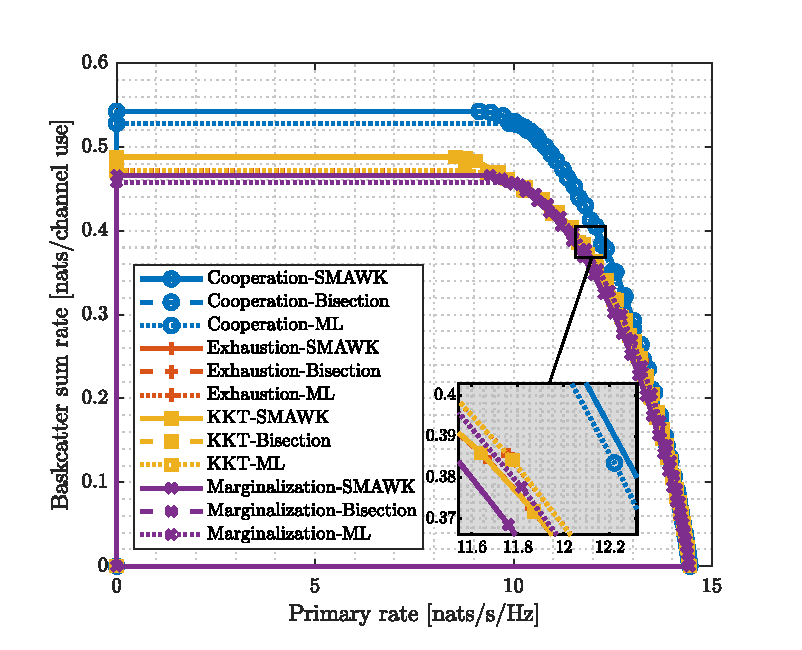
\includegraphics{assets/rate_region_1.eps}
		}
		\caption{Achievable rate regions by input-threshold design: Case I.}
		\label{fi:rate_region_1}
	\end{figure}

	\begin{figure}[!t]
		\centering
		\resizebox{\columnwidth}{!}{
			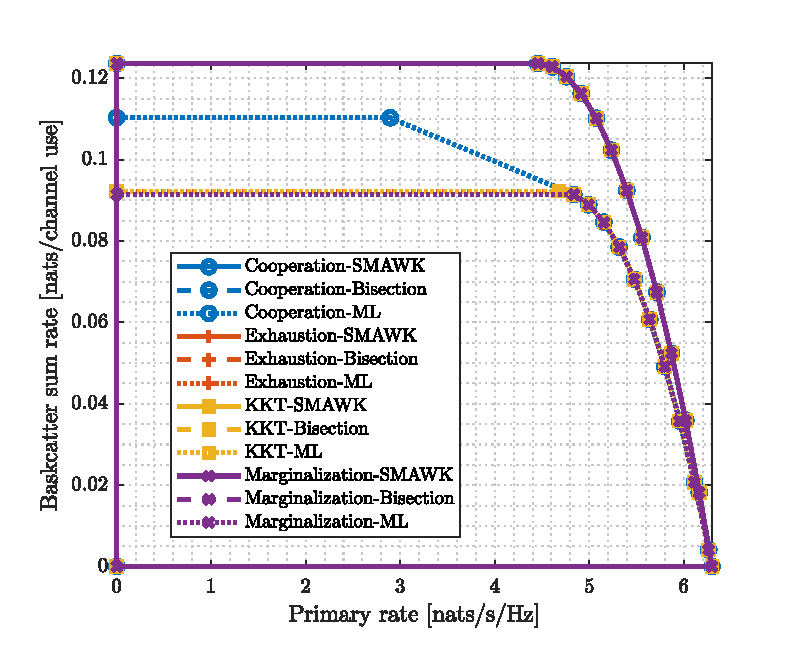
\includegraphics{assets/rate_region_2.eps}
		}
		\caption{Achievable rate regions by input-threshold design: Case II.}
		\label{fi:rate_region_2}
	\end{figure}
\end{section}

\begin{appendix}
	\begin{subsection}{Proof of Proposition \ref{pr:input_kkt_condition}}
		Denote the Lagrange multipliers associated with \eqref{co:sum_probability} and \eqref{co:nonnegative_probability} as $\{\nu_k\}_{k \in \mathcal{K}}$ and $\{\lambda_{k,m_k}\}_{k \in \mathcal{K},m_k \in \mathcal{M}}$, respectively.
		The Lagrangian function of problem \eqref{op:input_probability_distribution} is
		\begin{align}
			% L(\{\boldsymbol{p}_k\},\{\nu_k\},\{\lambda_{k,m_k}\})
			L
			 & = - I(x_{\mathcal{K}};\hat{x}_{\mathcal{K}},\boldsymbol{y}) + \sum_{k \in \mathcal{K}} \nu_k \left( \sum_{m_k \in \mathcal{M}} P_k(x_{m_k}) - 1 \right)\nonumber \\
			 & \quad - \sum_{k \in \mathcal{K}} \sum_{m_k \in \mathcal{M}} \lambda_{k,m_k} P_k(x_{m_k}),
		\end{align}
		and the \gls{kkt} conditions on the optimal primal and dual variables are, $\forall m_k \in \mathcal{M}$ and $\forall k \in \mathcal{K}$,
		\begin{subequations}
			\label{eq:input_kkt_condition_original}
			\begin{equation}
				- \nabla_{P_k^\star(x_{m_k})} I^\star(x_{\mathcal{K}};\hat{x}_{\mathcal{K}},\boldsymbol{y}) + \nu_k^\star - \lambda_{k,m_k}^\star = 0,
			\end{equation}
			\begin{equation}
				\lambda_{k,m_k}^\star = 0, \quad P_k^\star(x_{m_k}) > 0,
			\end{equation}
			\begin{equation}
				\lambda_{k,m_k}^\star \ge 0, \quad P_k^\star(x_{m_k}) = 0,
			\end{equation}
		\end{subequations}
		where the directional derivative can be explicitly expressed as
		\begin{equation}
			\nabla_{P_k^\star(x_{m_k})} I^\star(x_{\mathcal{K}};\hat{x}_{\mathcal{K}},\boldsymbol{y}) = I_k^\star(x_{m_k};\hat{x}_{\mathcal{K}},\boldsymbol{y}) - (1 - \rho).
			\label{eq:input_directional_derivative}
		\end{equation}

		Combining \eqref{eq:input_kkt_condition_original} and \eqref{eq:input_directional_derivative}, we have
		\begin{subequations}
			\label{eq:input_kkt_condition_transformed}
			\begin{alignat}{2}
				I_k^\star(x_{m_k};\hat{x}_{\mathcal{K}},\boldsymbol{y}) & = \nu_k^\star + (1 - \rho), \quad   &  & P_k^\star(x_{m_k}) > 0,\label{eq:probable_states_marginal} \\
				I_k^\star(x_{m_k};\hat{x}_{\mathcal{K}},\boldsymbol{y}) & \le \nu_k^\star + (1 - \rho), \quad &  & P_k^\star(x_{m_k}) = 0,\label{eq:dropped_states_marginal}
			\end{alignat}
		\end{subequations}
		which suggests
		\begin{equation}
			\sum_{m_k} P_k^\star(x_{m_k}) I_k^\star(x_{m_k};\hat{x}_{\mathcal{K}},\boldsymbol{y}) = \nu_k^\star + (1 - \rho).
			\label{eq:input_kkt_condition_implied}
		\end{equation}

		On the other hand, by definition of weighted sum marginal information \eqref{eq:weighted_sum_marginal_information},
		\begin{equation}
			\sum_{m_k} P_k^\star(x_{m_k}) I_k^\star(x_{m_k};\hat{x}_{\mathcal{K}},\boldsymbol{y}) = I^\star(x_{\mathcal{K}};\hat{x}_{\mathcal{K}},\boldsymbol{y}),
			\label{eq:weighted_sum_marginal_information_implied}
		\end{equation}
		where the right-hand side is irrelevant to $k$.
		\eqref{eq:input_kkt_condition_transformed}, \eqref{eq:input_kkt_condition_implied}, and \eqref{eq:weighted_sum_marginal_information_implied} together complete the proof.
		\qedsymbol
		\label{ap:input_kkt_condition}
	\end{subsection}

	\begin{subsection}{Proof of Proposition \ref{pr:input_kkt_solution}}
		We first prove sequence \eqref{eq:input_kkt_solution} is non-decreasing in mutual information.
		Let $P_{\mathcal{K}}(x_{m_{\mathcal{K}}}) = \prod_{q \in \mathcal{K}} P_q(x_{m_q})$ and $P_{\mathcal{K}}'(x_{m_{\mathcal{K}}}) = P_k'(x_{m_k}) \prod_{q \in \mathcal{K} \setminus \{k\}} P_q(x_{m_q})$ be two probability distributions with potentially different marginal for tag $k \in \mathcal{K}$ at state $m_k \in \mathcal{M}$, and define an intermediate function $J \left( P_{\mathcal{K}}(x_{m_{\mathcal{K}}}),P_{\mathcal{K}}'(x_{m_{\mathcal{K}}}) \right)$ as \eqref{eq:intermediate_information_function}.
		\begin{figure*}[!b]
			\hrule
			\begin{align}
				J \left( P_{\mathcal{K}}(x_{m_{\mathcal{K}}}),P_{\mathcal{K}}'(x_{m_{\mathcal{K}}}) \right)
				 & \triangleq \rho \sum_{m_{\mathcal{K}}} P_{\mathcal{K}}(x_{m_{\mathcal{K}}}) N \log_2 \left(1 + \frac{\lvert \boldsymbol{h}_{\mathrm{E}}^H(x_{m_{\mathcal{K}}}) \boldsymbol{w} \rvert^2}{\sigma_w^2}\right)\nonumber                                                                                                                          \\
				 & \quad + (1 - \rho) \sum_{m_{\mathcal{K}}} P_{\mathcal{K}}(x_{m_{\mathcal{K}}}) \sum_{m_{\mathcal{K}}'} P(\hat{x}_{m_{\mathcal{K}}'} \mid x_{m_{\mathcal{K}}}) \log \frac{P(\hat{x}_{m_{\mathcal{K}}'} \mid x_{m_{\mathcal{K}}}) P_{\mathcal{K}}'(x_{m_{\mathcal{K}}})}{P'(\hat{x}_{m_{\mathcal{K}}'}) P_{\mathcal{K}}(x_{m_{\mathcal{K}}})}.
				\label{eq:intermediate_information_function}
			\end{align}
		\end{figure*}
		It is straightforward to verify $J \left( P_{\mathcal{K}}(x_{m_{\mathcal{K}}}),P_{\mathcal{K}}(x_{m_{\mathcal{K}}}) \right) = I(x_{\mathcal{K}};\hat{x}_{\mathcal{K}},\boldsymbol{y})$ and $J \left( P_{\mathcal{K}}(x_{m_{\mathcal{K}}}),P_{\mathcal{K}}'(x_{m_{\mathcal{K}}}) \right)$ is a concave function for a fixed $P_{\mathcal{K}}'(x_{m_{\mathcal{K}}})$.
		By choosing $\nabla_{P_k^\star(x_{m_k})} J \left( P_{\mathcal{K}}(x_{m_{\mathcal{K}}}),P_{\mathcal{K}}'(x_{m_{\mathcal{K}}}) \right) = 0$, we have
		\begin{equation}
			S_k'(x_{m_k}) - S_k'(x_{i_k}) + (1 - \rho) \log \frac{P_k(x_{i_k})}{P_k^\star(x_{m_k})} = 0,
			\label{eq:optimal_intermediate_information_condition}
		\end{equation}
		where $i_k \ne m_k$ is the reference state and
		\begin{align}
			S_k'(x_{m_k})
			 & \triangleq I_k'(x_{m_k};\hat{x}_{\mathcal{K}},\boldsymbol{y}) + (1 - \rho) \sum_{m_{\mathcal{K} \setminus \{k\}}} P_{\mathcal{K} \setminus \{k\}}(x_{m_{\mathcal{K} \setminus \{k\}}})\nonumber \\
			 & \quad \times \sum_{m_{\mathcal{K}}'} P(\hat{x}_{m_{\mathcal{K}}'} \mid x_{m_{\mathcal{K}}}) \log P_{\mathcal{K}}'(x_{m_{\mathcal{K}}}).
		\end{align}

		Evidently, $\forall m_k \ne i_k$, \eqref{eq:optimal_intermediate_information_condition} boils down to
		\begin{equation}
			P_k^\star(x_{m_k}) = \frac{P_k'(x_{m_k}) \exp \left( \frac{\rho}{1 - \rho} I_k'(x_{m_k};\hat{x}_{\mathcal{K}},\boldsymbol{y}) \right)}{\sum_{m_k'} P_k'(x_{m_k'}) \exp \left( \frac{\rho}{1 - \rho} I_k'(x_{m_k'};\hat{x}_{\mathcal{K}},\boldsymbol{y}) \right)}.
			\label{eq:optimal_relative_distribution}
		\end{equation}

		Although it seems $P_k(x_{i_k}) = 1 - \sum_{m_k \ne i_k} P_k^\star(x_{m_k})$ has no optimality guarantee, we can verify that $P_k(x_{i_k})$ has exactly the same form as \eqref{eq:optimal_relative_distribution}.
		It implies the selection of reference state does not matter and \eqref{eq:optimal_relative_distribution} is indeed optimal $\forall m_k \in \mathcal{M}$.
		Therefore, for a fixed $P_{\mathcal{K}}'(x_{m_{\mathcal{K}}})$, choosing $P_k(x_{m_k})$ by \eqref{eq:optimal_relative_distribution} ensures
		\begin{equation}
			J \left( P_{\mathcal{K}}(x_{m_{\mathcal{K}}}),P_{\mathcal{K}}'(x_{m_{\mathcal{K}}}) \right) \ge I'(x_{\mathcal{K}};\hat{x}_{\mathcal{K}},\boldsymbol{y}).
			\label{eq:information_difference_lower}
		\end{equation}

		On the other hand, \eqref{eq:optimal_relative_distribution} also guarantees
		\begin{subequations}
			\label{eq:information_difference_upper}
			\begin{align}
				\Delta
				 & \triangleq I(x_{\mathcal{K}};\hat{x}_{\mathcal{K}},\boldsymbol{y}) - J \left( P_{\mathcal{K}}(x_{m_{\mathcal{K}}}),P_{\mathcal{K}}'(x_{m_{\mathcal{K}}}) \right)                                                                                                                               \\
				 & = (1 - \rho) \sum_{m_k} \frac{P_k'(x_{m_k}) f_k'(x_{m_k};\hat{x}_{\mathcal{K}},\boldsymbol{y})}{\sum_{m_k'} P_k'(x_{m_k'}) f_k'(x_{m_k'};\hat{x}_{\mathcal{K}},\boldsymbol{y})} \sum_{m_{\mathcal{K}}''} P(\hat{x}_{m_{\mathcal{K}}''} \mid x_{m_k})\nonumber                                  \\
				 & \quad \times \log \frac{\sum_{m_k'} P_k'(x_{m_k'}) P(\hat{x}_{m_{\mathcal{K}}''} \mid x_{m_k'}) f_k'(x_{m_k};\hat{x}_{\mathcal{K}},\boldsymbol{y})}{\sum_{m_k'} P_k'(x_{m_k'}) P(\hat{x}_{m_{\mathcal{K}}''} \mid x_{m_k'}) f_k'(x_{m_k'};\hat{x}_{\mathcal{K}},\boldsymbol{y})}               \\
				 & \ge (1 - \rho) \sum_{m_k} \frac{P_k'(x_{m_k}) f_k'(x_{m_k};\hat{x}_{\mathcal{K}},\boldsymbol{y})}{\sum_{m_k'} P_k'(x_{m_k'}) f_k'(x_{m_k'};\hat{x}_{\mathcal{K}},\boldsymbol{y})} \sum_{m_{\mathcal{K}}''} P(\hat{x}_{m_{\mathcal{K}}''} \mid x_{m_k})\nonumber                                \\
				 & \quad \times \left( 1 - \frac{\sum_{m_k'} P_k'(x_{m_k'}) P(\hat{x}_{m_{\mathcal{K}}''} \mid x_{m_k'}) f_k'(x_{m_k'};\hat{x}_{\mathcal{K}},\boldsymbol{y})}{\sum_{m_k'} P_k'(x_{m_k'}) P(\hat{x}_{m_{\mathcal{K}}''} \mid x_{m_k'}) f_k'(x_{m_k};\hat{x}_{\mathcal{K}},\boldsymbol{y})} \right) \\
				 & = 0,
			\end{align}
		\end{subequations}
		where $f_k'(x_{m_k};\hat{x}_{\mathcal{K}},\boldsymbol{y}) \triangleq \exp \left( \frac{\rho}{1 - \rho} I_k'(x_{m_k};\hat{x}_{\mathcal{K}},\boldsymbol{y}) \right)$ and the equality holds if and only if \eqref{eq:optimal_relative_distribution} converges.
		\eqref{eq:information_difference_lower} and \eqref{eq:information_difference_upper} together imply $I(x_{\mathcal{K}};\hat{x}_{\mathcal{K}},\boldsymbol{y}) \ge I'(x_{\mathcal{K}};\hat{x}_{\mathcal{K}},\boldsymbol{y})$.
		Since mutual information is bounded above, we conclude the sequence \eqref{eq:input_kkt_solution} is non-decreasing and convergent in mutual information.

		Next, we prove that any converging point of sequence \eqref{eq:input_kkt_solution}, denoted as $P_k^\star(x_{m_k})$, fulfills \gls{kkt} conditions \eqref{eq:input_kkt_condition}.
		To see this, consider $P_k^{(0)}(x_{m_k}) > 0$ and define
		\begin{equation}
			D_k^{(r)}(x_{m_k}) \triangleq \frac{P_k^{(r+1)}(x_{m_k})}{P_k^{(r)}(x_{m_k})} = \frac{f_k^{(r)}(x_{m_k};\hat{x}_{\mathcal{K}},\boldsymbol{y})}{\sum_{m_k'} P_k^{(r)}(x_{m_k'}) f_k^{(r)}(x_{m_k'};\hat{x}_{\mathcal{K}},\boldsymbol{y})}.
		\end{equation}

		As sequence \eqref{eq:input_kkt_solution} is convergent, any state with $P_k^\star(x_{m_k}) > 0$ need to satisfy $D_k^\star(x_{m_k}) \triangleq \lim_{r \to \infty} D_k^{(r)}(x_{m_k}) = 1$, namely
		\begin{equation}
			I_k^\star(x_{m_k};\hat{x}_{\mathcal{K}},\boldsymbol{y}) = \frac{1 - \rho}{\rho} \log \sum_{m_k'} P_k^\star(x_{m_k'}) f_k^\star(x_{m_k'};\hat{x}_{\mathcal{K}},\boldsymbol{y}),
		\end{equation}
		which is reminiscent of \eqref{eq:probable_states_marginal} (and hence \eqref{eq:probable_states}).
		That is to say, given $P_k^{(0)}(x_{m_k}) > 0$, any converging point with $P_k^\star(x_{m_k}) > 0$ must satisfy \eqref{eq:probable_states}.
		On the other hand, we assume $P_k^\star(x_{m_k})$ does not satisfy \eqref{eq:dropped_states}, such that for any state with $P_k^\star(x_{m_k}) = 0$,
		% On the other hand, we show if $P_k^\star(x_{m_k})$ does not satisfy \eqref{eq:dropped_states}, then it is not a converging point of sequence \eqref{eq:input_kkt_solution}. By this assumption, for any state with $P_k^\star(x_{m_k}) = 0$,
		\begin{equation}
			I_k^\star(x_{m_k};\hat{x}_{\mathcal{K}},\boldsymbol{y}) > I^\star(x_{\mathcal{K}};\hat{x}_{\mathcal{K}},\boldsymbol{y}) = \sum_{m_k'} P_k^\star(x_{m_k'}) I_k^\star(x_{m_k'};\hat{x}_{\mathcal{K}},\boldsymbol{y}),
		\end{equation}
		where the equality inherits from \eqref{eq:weighted_sum_mutual_information}.
		Since the exponential function is monotonically increasing, we have $f_k^\star(x_{m_k};\hat{x}_{\mathcal{K}},\boldsymbol{y}) > \sum_{m_k'} P_k^\star(x_{m_k'}) f_k^\star(x_{m_k'};\hat{x}_{\mathcal{K}},\boldsymbol{y})$ and $D_k^\star(x_{m_k}) > 1$.
		Considering $P_k^{(0)}(x_{m_k}) > 0$ and $P_k^\star(x_{m_k}) = 0$, it contradicts with
		\begin{equation}
			P_k^{(r)}(x_{m_k}) = P_k^{(0)}(x_{m_k}) \prod_{n=1}^r D_k^{(n)}(x_{m_k}).
		\end{equation}
		Therefore, given $P_k^{(0)}(x_{m_k}) > 0$, any converging point with $P_k^\star(x_{m_k}) = 0$ must satisfy \eqref{eq:dropped_states}.
		This completes the proof.
		\qedsymbol
		\label{ap:input_kkt_solution}
	\end{subsection}

	\begin{subsection}{Proof of Proposition \ref{pr:threshold}}
		Since $L$ input letters are with non-zero probability and $x \to z \to \hat{x}$ formulates a Markov chain, we need $L$ non-empty decision regions and at least $L+1$ distinct thresholds (including \num{0} and $\infty$) to minimize the distortion between source and decision.
		On the other hand, the optimal decision regions are apparently empty for those unused letters.

		Suppose the optimal number of thresholds is $S+1$ where $S \ge L$.
		Let $\boldsymbol{t} \triangleq [t_0,\ldots,t_S]^T \in \mathbb{R}_{+}^{(S+1) \times 1}$ be the optimal threshold vector where $t_{s-1} < t_s$, $\forall s \in \mathcal{S} \triangleq \{1,\ldots,S\}$.
		Since the optimal decision region for any letter may consist of multiple partitions, without loss of generality, we assume the mapping from threshold vector to decision region $l' \in \mathcal{L} \triangleq \{1,\ldots,L\}$ is given by $\mathcal{R}_{l'} = \bigcup_{s \equiv l' \pmod L} [t_{s-1},t_s)$.
		\begin{footnote}
			The proof holds for any valid mapping from threshold vector to decision regions, and we consider this specific case for the ease of presentation.
		\end{footnote}
		The threshold optimization problem is
		\begin{maxi!}
			{\scriptstyle{\boldsymbol{t}}}{I_{\mathrm{B}}(x;\hat{x})}{\label{op:decision_threshold}}{\label{ob:backscatter_mutual_information}}
			\addConstraint{t_{s-1}}{< t_s,}{\quad \forall s \in \mathcal{S}.}{\label{co:strict_inequality}}
		\end{maxi!}

		Problem \eqref{op:decision_threshold} is intricate due to the strict inequality constraint \eqref{co:strict_inequality}.
		Following \cite{Nguyen2020}, we first relax it to the convex counterpart, then discard the solutions that violate any original constraint.
		The Lagrangian function for the relaxed problem is
		\begin{equation}
			L = - I_{\mathrm{B}}(x;\hat{x}) + \sum_{s \in \mathcal{S}} \mu_s (t_{s-1} - t_s),
		\end{equation}
		where $\mu_s$ is the Lagrange multiplier associated with the non-strict version of \eqref{co:strict_inequality}.
		The \gls{kkt} conditions on the optimal primal and dual solutions are, $\forall s \in \mathcal{S}$,
		\begin{subequations}
			\label{eq:kkt_thresholding}
			\begin{equation}
				- \nabla_{t_s^\star} I^\star_{\mathrm{B}}(x;\hat{x}) + \mu_{s-1}^\star - \mu_s^\star = 0,
				\label{eq:stationarity}
			\end{equation}
			\begin{equation}
				\mu_s^\star \ge 0,
				\label{eq:dual_feasibility}
			\end{equation}
			\begin{equation}
				\mu_s^\star (t_{s-1}^\star - t_s^\star) = 0.
				\label{eq:complementary_slackness}
			\end{equation}

		\end{subequations}
		Due to the strict inequality constraint \eqref{co:strict_inequality}, conditions \eqref{eq:dual_feasibility} and \eqref{eq:complementary_slackness} together imply $\mu_s^\star = 0$, $\forall s \in \mathcal{S}$.
		Besides, it is trivial to conclude $t_0^\star = 0$ for energy-based detection.
		As such, the necessary optimality conditions for problem \eqref{op:decision_threshold}, $\forall s \in \mathcal{S}$,
		\begin{equation}
			\nabla_{t_{s}^\star} I^\star_{\mathrm{B}}(x;\hat{x}) = 0,
		\end{equation}
		which can be explicitly written as, $\forall s \equiv l' \pmod L$,
		\begin{equation}
			\sum_l P(x_l) \frac{(t_s^\star)^{N-1} e^{-t_s^\star/\sigma_l^2}}{\sigma_l^{2N} (N-1)!} \log \frac{P(x_l \mid \hat{x}_{l'+1})}{P(x_l \mid \hat{x}_{l'})} = 0,
			\label{eq:kkt_threshold_explicit}
		\end{equation}

		According to \cite{He2021}, the optimal backward channel quantizer is convex and separates each pair of posterior distribution by a hyperplane.
		It implies, for a given output letter $l'$, the sequence $\{\log {P(x_l \mid \hat{x}_{l'+1})}/{P(x_l \mid \hat{x}_{l'})}\}_{l \in \mathcal{L}}$ changes sign exactly once.
		We notice the left-hand side of \eqref{eq:kkt_threshold_explicit} is a generalized Dirichlet polynomial, and by Descartes' rule of signs \cite{Jameson2006}, has at most one positive solution.
		% TODO
		In other words, starting from $t_0^\star$, each optimal decision region requires at most one additional distinct threshold, and we have $S \le L$.
		Therefore, we conclude $S = L$ and the proof is completed.
		\qedsymbol
		\label{ap:threshold}
	\end{subsection}
\end{appendix}


\bibliographystyle{IEEEtran}
\bibliography{library.bib}
\end{document}
